\documentclass[12pt]{jreport}
\renewcommand{\bibname}{参考文献} 
\usepackage[dvipdfmx]{graphicx}
\usepackage{ascmac,url,moreverb,multirow,style/eclbkbox,fancybox,enumerate,bxbase,inputenc,listings}
\setlength{\textheight}{25cm}		%1ページ当りの行数を指定する
\setlength{\textwidth}{38zw}		%1行あたりの文字数の設定
\setlength{\evensidemargin}{10mm}   %偶数ページの余白
\setlength{\oddsidemargin}{10mm}    %奇数ページの余白
\setlength{\topmargin}{-3mm}        %上の余白
\setlength{\headheight}{0mm}        %ヘッダ領域の高さ
\setlength{\headsep}{0mm}           %ヘッダ領域と本文領域との間隔
\setlength{\columnsep}{12mm}        %段組にした場合の段同士の間隔
\setlength{\footskip}{10mm}         %フッタ領域と本文との間隔
\setlength{\belowcaptionskip}{5pt}
%macro setting

%画像用マクロ
\newenvironment{img}[0]
{
\begin{figure}[!h]
\begin{screen}
\begin{center}
}{
\end{center}
\end{screen}
\end{figure}
}


%コマンド表示用 
\newenvironment{cmd}[0]
{
\begin{screen}
}{
\end{screen}
}

%スクリプト表示
\newenvironment{script}{
\VerbatimEnvironment
\begin{breakbox}
\small
\begin{Verbatim}
}{
\end{Verbatim}
\normalsize
\end{breakbox}
}					%マクロの読み込み
%%%%%%%%%%%%%%%%%%%%%%%%%%%%%%%%%%%%%%%%%%%%%%%%%%%%%%%%%%%%%%%%%%%%%%%

\title{AIを用いた楽曲制作に関する検討}					%卒業論文タイトル
\author{1532117 秋場  翼\\1532151 松元 孝樹\\\normalsize 指導教員:中村 直人 教授}	%名前(苗字と名前は全角1字空け)
\date{平成31年度}                   %日付設定(デフォルトは現在の年月日)

%%%%%%%%%%%%%%%%%%%%%%%%%%%%%%%%%%%%%%%%%%%%%%%%%%%%%%%%%%%%%%%%%%%%%%%
\begin{document}
\pagenumbering{roman}
\maketitle                        	%タイトルをドキュメントへ貼り付け
\tableofcontents               	%目次を作成
\listoffigures				%図の目次作成
\listoftables				%表の目次作成

\baselineskip 20pt              	%行間設定

\clearpage
\pagenumbering{arabic}


%ここから内容

%\input{ディレクトリ名/ファイル名}

\chapter{序論}
\section{研究の背景と目的}
近年,AI分野は急速な発展を続けている.スマートスピーカなどの対話型のAIがGoogleやAmazon,IBMによって商品化され,現在ではスマートフォンにもSiriというAIが搭載されるなどその存在は非常に身近になっており,その種類も非常に多岐にわたる.
\begin{figure}[h]
    \begin{screen}
    \begin{center}
        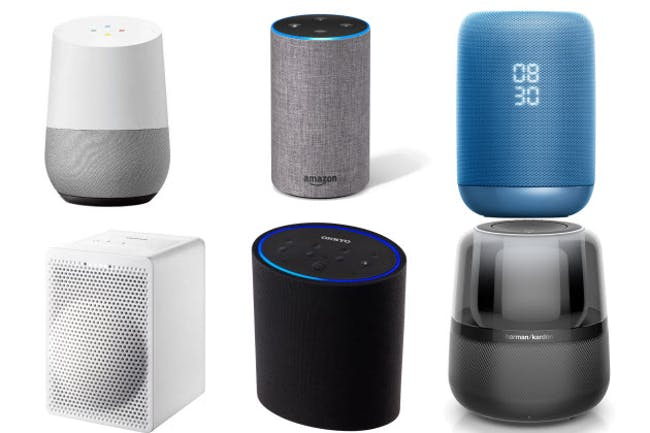
\includegraphics[scale=0.6, clip]{./img/smartspeaker_list.jpg}
        \caption{magentaによるMIDI音楽データ生成までのプロセス}
        \label{fig:magentaによるMIDI音楽データ生成までのプロセス}
    \end{center}
\end{screen}
\end{figure}\\
また囲碁や将棋,チェスなどの競技においても,プロにAIが勝利するなどその精度は以前から高いが,そのAIは一つの競技でしか使用できない特化型人工知能(AGI)でありった.
しかし,英DeepMindが発表したAlphaZeroという様々なボードゲームに対応できる汎用性を持ったAIが発表され,汎用人工知能(GAI)の成長も著しい.\\
自然言語処理を用いた芸術の分野では,2012年にスタートした人工知能を使って小説を生成するプロジェクトが「星新一賞」の第一審査を通過した.
また,絵画や音楽に関してもAIが作成した肖像画が米競売大手クリスティーズのオークションで43万2500ドル(約4900万円)で落札され,AIを用いて新しい作品を作るものが出回っている.\\
 このようにAIの発展は様々な分野においてその成果を上げており,今後は業務の効率化や補助だけにとどまらず,自動車の自動運転や医療の現場でも人間の手よりも高精度なものとして活躍することが期待されている.\\
本研究ではAIによる楽曲生成についての実証実験を行う.
Googole brainによって公開されているTensorflowのライブラリであるMagentaはAI Duetや
そのライブラリを用いて学習データやノード数による楽曲の生成結果の違いを比較,検証し,AIによる楽曲制作が有用なものか調査する.\\
\section{本論文の構成}
本論文の構成は以下の通りである.\\
第1章では本論文の背景と目的について述べている.\\
第2章では本論文で利用する理論について述べている.\\
第3章では実験内容について述べている.\\
第4章では楽曲制作について述べている.\\
第5章ではAIを用いた楽曲制作についての本研究の結論について述べている.\\
\chapter{理論}
\section{AIを用いた楽曲作成}
\subsection{MIDI}
%MIDIとオーディオデータの形式について述べる
パソコンで用いる音楽データには大きく分けて二つある.一つ目はオーディオデータといい波形の情報を記録する形式である.二つ目がMIDIである.\\
 AIによる曲制作では主にMIDIファイルの音楽データを使用する.MIDIファイルは実際の音ではなく音楽の演奏情報(音の高さや長さなど)である.
本研究で用いるAIはこのMIDIファイルの情報を元に学習をする.また入出力の際もこの規格を用いる.\\
 なお,インプットデータはone-hot Vectorで図\ref{fig:インプットデータの仕組み}のようになっている.また,楽曲制作の際に音程を指定する場合は図\ref{fig:MIDIと音階}の数値を指定する.
\begin{figure}[h]
    \begin{screen}
    \begin{center}
        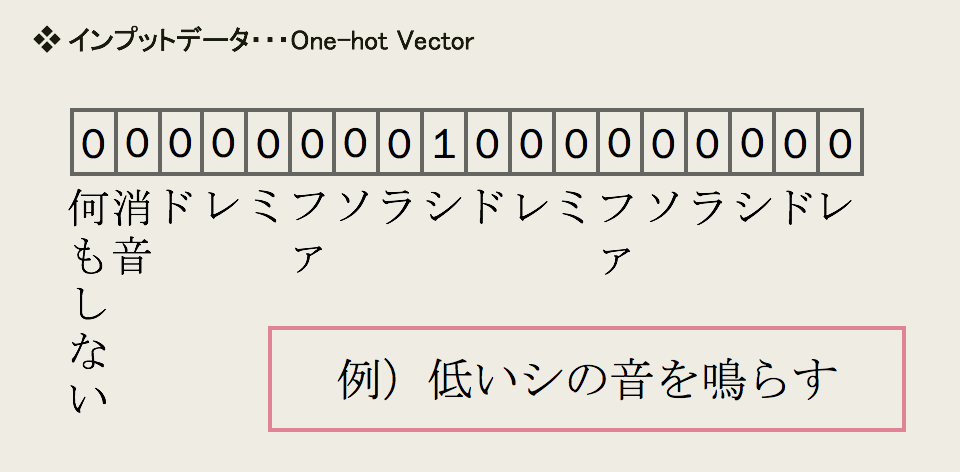
\includegraphics[scale=0.8,clip]{./img/midi1.png}
        \caption{インプットデータの仕組み}
        \label{fig:インプットデータの仕組み}
    \end{center}
    \end{screen}
\end{figure}
\newpage
\begin{figure}[h]
    \begin{screen}
    \begin{center}
        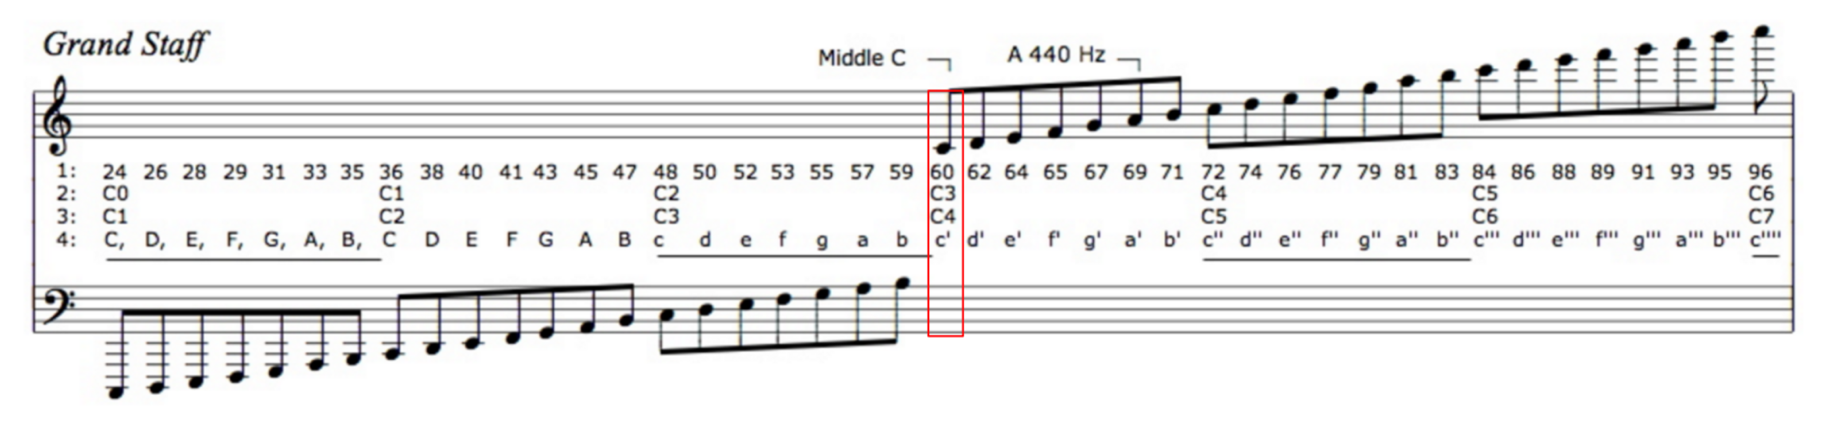
\includegraphics[scale=0.4,clip]{./img/midi2.png}
        \caption{MIDIと音階}
        \label{fig:MIDIと音階}
    \end{center}
    \end{screen}
\end{figure}
%AIを用いた楽曲サービスについて述べてその中でなぜMagendaを選ぶのかを述べる
\subsection{Magenta}
本研究で使用するMagentaは音楽などをTensorFlowを使って機械学習するライブラリであり,Google BrainがGitHab上に公開されているOSSである.
Magentaではまず学習させたい音楽のMIDIデータをNoteSequence(magentaが扱うファイル形式)とよばれるデータフォーマットに変更する.それを学習用データセットと評価用データセットに変換したあと学習を行う.
このとき,一度に学習させるデータの数,学習を行う回数,ノード数を設定する.これをパッケージ化し,MIDIファイルとして新たに楽曲を生成するという流れである.これを図2.1に示す.
\begin{figure}[h]
    \begin{screen}
    \begin{center}
        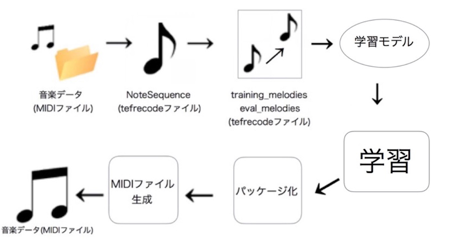
\includegraphics[scale=1.7, clip]{./img/magenta_usestep.png}
        \caption{magentaによるMIDI音楽データ生成までのプロセス}
        \label{fig:magentaによるMIDI音楽データ生成までのプロセス}
    \end{center}
    \end{screen}
\end{figure}
\section{機械学習に適した開発環境について}
MagendaでTensolflowのライブラリである.
Tensolflowのランタイムとして以下のシステムがサポートされている.
\begin{enumerate}
    \renewcommand{\labelenumi}{(\arabic{enumi})}
    \item Ubuntu 16.04以降
    \item macOS 10.12.6(Sierra)以降(GPUサポートなし)
    \item Windows7 以降
    \item Raspbian 9.0以降
\end{enumerate}
また,GPUを用いて学習を行う時にはtensolflow-gpuというパッケージが必要となり,導入には以下のドライバやライブラリが必要である.
\begin{enumerate}
    \renewcommand{\labelenumi}{(\arabic{enumi})}
    \item CUDA Toolkit (tensolflowはCUDA9.0をサポート)
    \item CUPTI (CUDA Toolkitに付随)
    \item NVIDEAGPUドライバ(CUDA9.0には384.x以上が必要)
    \item cuDNN SDK
\end{enumerate}
以上の事を踏まえて今研究では学習回数が多いため,GPUサポートのないmacOSは除く.
また,Windows10の環境ではリリースされているCUDAのバージョンは10のみであり,Tensolflowのサポートを外れてしまう.
そのため,CUDAv9がインストール可能なUbuntuを用いることとし,システムの開発環境を表\ref{tab:開発環境}に示す.
    \begin{table}[h]
    \begin{center}
    \caption{開発環境}
    \label{tab:開発環境}
    \begin{tabular}{|c|p{20zw}|}
    \hline
        OS & Ubuntu 16.04 LTS\\
        \hline
        CPU & Intel Core i3 8100\\
        \hline
        メモリ & 8GB\\
        \hline
        GPU & GeForce GTX 1060\\
        \hline
        CUDA & CUDA(9),cuDNN(7.4.2)\\
        \hline
        ライブラリ & TensorFlow(1.12.0),magenta(0.5.0)\\
        \hline
    \end{tabular}
    \end{center}
    \end{table}\\
\subsection{CUDA}
CUDAは、NVIDIAが開発しているGPU上でプログラミングをするためのソフトウェアプラットフォームになる.
含まれるものとしては、CUDAを実行形式に変えるコンパイラや、それをサポートするSDK、ライブラリ、あとはデバッグツール群である.
CUDAを導入することによって、プログラムを単に複数のプロセッサで動かすだけでなく、無駄なく並列化することができる。
\chapter{実験内容}
\section{モデルによる違い}
本研究ではMagentaで用意されている2つの学習モデルを用いた。以下に示すモデルを用いて楽曲制作をそれぞれ行い,比較,検証する.
\subsection{MelodyRNN}
MelodeRNNは楽曲のメロディを制作するモデルである.MelodyRNNである3つのモデルを以下に示す.\\
(1) basic\_rnn\\
 前の状態を保持し,これを記憶または忘却する.時系列を学習することにより,次の音の予測を可能にしている.Lookback\_rnnとAttention\_rnnはこれを基に機能を追加したものである.
\begin{figure}[!ht]
    \begin{screen}
    \begin{center}
        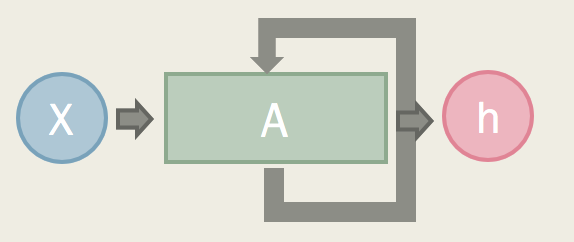
\includegraphics[scale=1, clip]{./img/basic3.png}
        \caption{basicrnnのモデル1}
        \label{fig:basicrnnのモデル1}
    \end{center}
    \end{screen}
\end{figure}\\
\newpage
\begin{figure}[!ht]
    \begin{screen}
    \begin{center}
        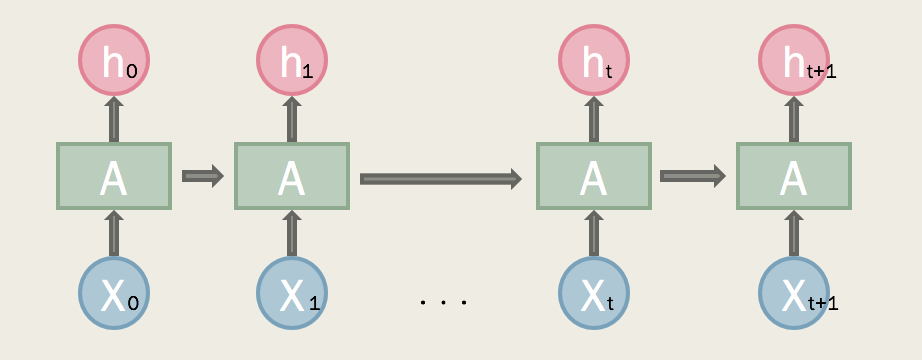
\includegraphics[scale=0.8, clip]{./img/basic4.png}
        \caption{basicrnnのモデル2}
        \label{fig:basicrnnのモデル2}
    \end{center}
    \end{screen}
\end{figure}\\
 Lookback\_rnnとAttention\_rnnはこれを基に機能を追加したものである
\begin{figure}[!ht]
    \begin{screen}
    \begin{center}
        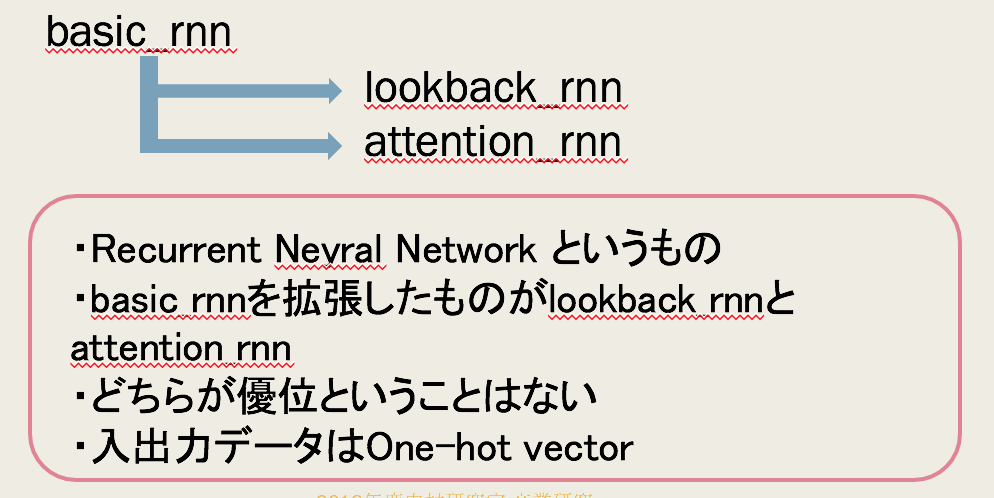
\includegraphics[scale=0.8, clip]{./img/basic1.png}
        \caption{三つのモデルについて}
        \label{fig:MelodyRNNについて}
    \end{center}
    \end{screen}
\end{figure}\\
\newpage
(2) lookback\_rnn\\
 Basic\_rnnを基に,1小節前と2小節前の音,拍数,前の小節の繰り返しかどうかの情報を与え,音楽の流れを掴もうとするもの.\\
\begin{figure}[!ht]
    \begin{screen}
    \begin{center}
        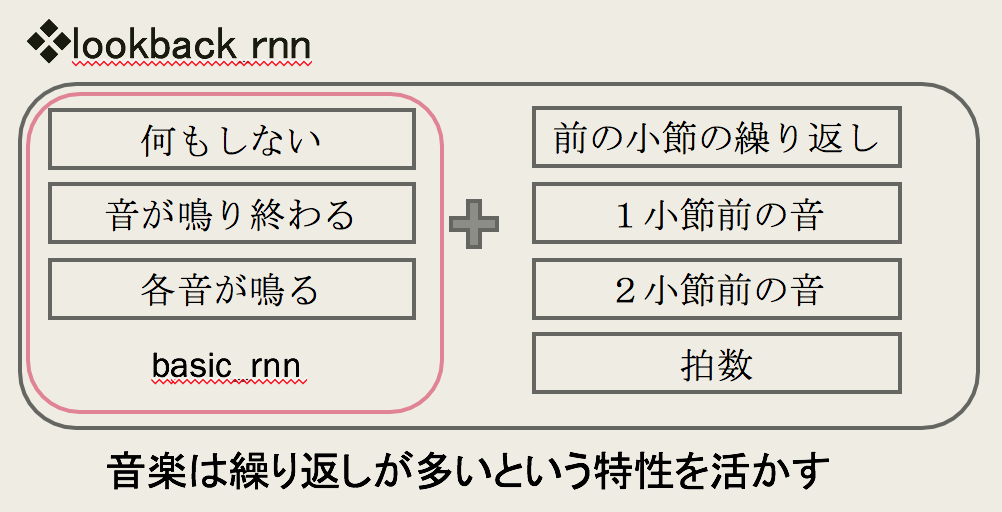
\includegraphics[scale=0.8, clip]{./img/lookback1.png}
        \caption{lookbackrnnのモデル}
        \label{fig:lookbackrnnのモデル}
    \end{center}
    \end{screen}
\end{figure}\\
\newpage
(3) attention\_rnn\\
 basic\_rnnを基に,過去の情報を予測結果に加えてこれによる繰り返しを捉えるもの.\\
\begin{figure}[!ht]
    \begin{screen}
    \begin{center}
        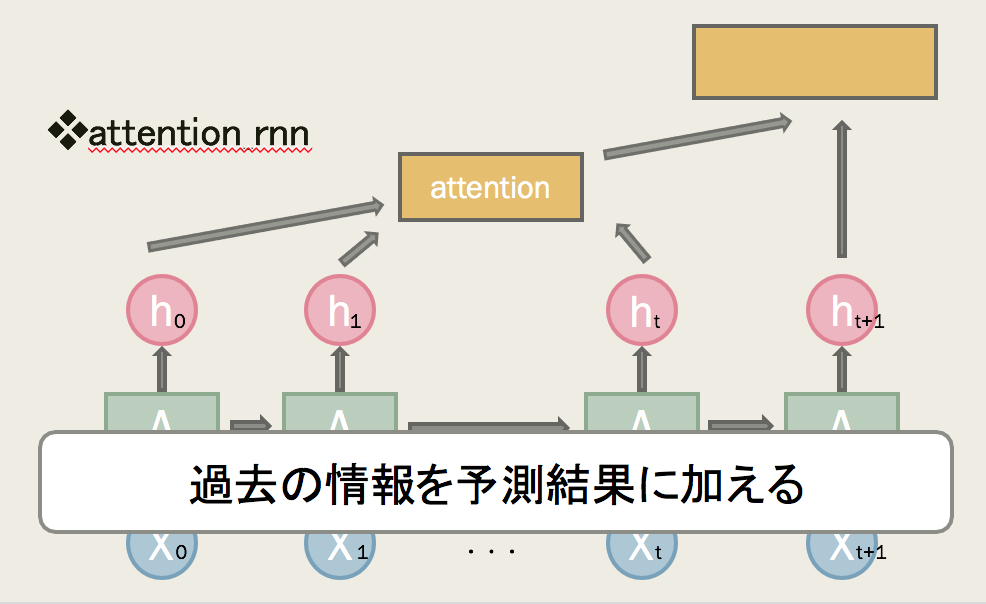
\includegraphics[scale=0.8, clip]{./img/attention1.png}
        \caption{attentionrnnのモデル}
        \label{fig:attentionrnnのモデル}
    \end{center}
    \end{screen}
\end{figure}\\
\subsection{PolyphonyRNN}
 複数の同時音のモデリングが可能になっており,複数音の響きを1つのかたまりとして捉えて学習しているモデルである.このモデルを使用することで,伴奏も含めた楽曲の生成が可能である\\
上記のモデルを用いて制作を行い,それぞれの違いと有用性について検証する.
\section{学習回数による違い}
 学習回数を変更して楽曲制作を行い,それぞれの違いと有用性について検証する.
\section{ノード数による違い}
 ノード数を変更して楽曲制作を行い,それぞれの違いと有用性について検証する.
\chapter{楽曲制作}
\section{Melody\_rnnを使用して学習モデルを作成}
\subsection{NoteSequenceの作成}
NoteSequenceとはMIDIデータから作成されるプロトコルバッファである.
プロトコルバッファとはGoogleが2008年にオープンソース化したバイナリベースのデータフォーマットである.
既存の技術としてはXMLやJSONなどのテキストベースのデータフォーマットがあるが,プロトコルバッファはバイナリフォーマットであるので,アプリケーション間でデータ構造の送受信をする際に少ないデータ量ですむという特徴がある.
また,シリアライズ化された情報をデシリアライズする速度もJSONよりもプロトコルバッファの方が早い.
しかし,データはバイナリ形式であるため,デシリアライズしなければ読むことができないため,JSONと比べて可読性は低い.
\begin{table}[h]
\begin{center}
\caption{JSONとプロトコルバッファの比較}
\label{tab:JSONとプロトコルバッファの比較}
\begin{tabular}{|l|c|c|}
\hline
    プロトコルバッファ & JSON\\ \hline
    \hline
    フォーマット & バイナリベース & テキストベース\\
    \hline
    データ量 & 少ない & 多い\\
    \hline
    可読性 & 低い & 高い\\
    \hline
    デシリアライズ & 高速 & 低速\\
    \hline
\end{tabular}
\end{center}
\end{table}
 NoteSequenceの作成は以下に示すコマンドで作成できる.\\
 --input\_dirで学習させるMIDIデータのディレクトリの絶対パスを指定し,--output\_fileでNotesequenceの出力先のディレクトリを指定する.\\
\begin{lstlisting}[basicstyle=\ttfamily\footnotesize,frame=single]
    convert\_dir\_to\_note\_sequences \
    --input\_dir=\$INPUT\_DIRECTORY \
    --output\_file=\$SEQUENCES\_TFRECORD \
    --recursive
\end{lstlisting}
\newpage
次に作成したNoteSequenceのデータセットを学習用と評価用に分割するために以下に示すのコマンドを実行する.\\
 --configで使用するRNNを指定する.--input\_dirでNoteSequenceの絶対パスを指定し,--output\_fileで分割したNotesequenceの出力先のディレクトリを指定する.
--eval\_ratioでNotesequenceのデータを何パーセント学習用に用いるかを指定する.コマンドの場合は10\%が学習用のデータになる.
\begin{lstlisting}[basicstyle=\ttfamily\footnotesize,frame=single]
melody_rnn_create_dataset \
--config=<one of 'basic_rnn', 'lookback_rnn', or 'attention_rnn'> \
--input=/tmp/notesequences.tfrecord \
--output_dir=/tmp/melody_rnn/sequence_examples \
--eval_ratio=0.10
\end{lstlisting}
\subsection{basic\_rnnを用いて学習を開始}
作成したNoteSequenceから学習モデルを作成するために以下のコマンドを実行する.\\
--configで学習に使用するbasic\_rnnを指定,--rundirで学習のために用意したNotesequenceを指定し,--sequence\_examplefileで学習モデルの出力先のディレクトリを指定する.
--hparamsでメモリの使用量を指定し,--rnn\_layer\_sizeで中間層のノード数を指定し,--num\_trainingstepsで学習回数を設定する.\\
\begin{lstlisting}[basicstyle=\ttfamily\footnotesize,frame=single]
melody_rnn_train \
--config=basic_rnn \
--run_dir=/tmp/melody_rnn/logdir/run1 \
--sequence_example_file=/tmp/melody_rnn/training_melodies.tfrecord \
--hparams="batch_size=64,rnn_layer_sizes=[64,64]" \
--num_training_steps=20000
\end{lstlisting}
\newpage
\subsection{lookback\_rnnを用いて学習を開始}
作成したNoteSequenceから学習モデルを作成するために以下のコマンドを実行する.\\
 --configで学習に使用するlookback\_rnnを指定,--rundirで学習のために用意したNotesequenceを指定し,--sequence\_examplefileで学習モデルの出力先のディレクトリを指定する.
--hparamsでメモリの使用量を指定し,--rnn\_layer\_sizeで中間層のノード数を指定し,--num\_trainingstepsで学習回数を設定する.\\
\begin{lstlisting}[basicstyle=\ttfamily\footnotesize,frame=single]
melody_rnn_train \
--config=lookback_rnn \
--run_dir=/tmp/melody_rnn/logdir/run1 \
--sequence_example_file=/tmp/melody_rnn/training_melodies.tfrecord \
--hparams="batch_size=64,rnn_layer_sizes=[64,64]" \
--num_training_steps=20000
\end{lstlisting}

\subsection{attention\_rnnを用いて学習を開始}
作成したNoteSequenceから学習モデルを作成するために以下のコマンドを実行する.\\
 --configで学習に使用するattention\_rnnを指定,--rundirで学習のために用意したNotesequenceを指定し,--sequence\_examplefileで学習モデルの出力先のディレクトリを指定する.
--hparamsでメモリの使用量を指定し,--rnn\_layer\_sizeで中間層のノード数を指定し,--num\_trainingstepsで学習回数を設定する.\\
\begin{lstlisting}[basicstyle=\ttfamily\footnotesize,frame=single]
melody_rnn_train \
--config=attention_rnn \
--run_dir=/tmp/melody_rnn/logdir/run1 \
--sequence_example_file=/tmp/melody_rnn/training_melodies.tfrecord \
--hparams="batch_size=64,rnn_layer_sizes=[64,64]" \
--num_training_steps=20000
\end{lstlisting}
\newpage
\subsection{basic\_rnnを用いて音楽データの作成}
以下に示すコマンドで学習モデルに入力する.\\
 --configで学習に使用するbasic\_rnnを指定,--rundirで学習済みのモデルを指定し,--output\_dirで音楽データの出力先のディレクトリを指定する.
--num\_outputsで生成する音楽データの個数を指定し,--num\_stepsで
--hparamsでメモリの使用量を指定し,--rnn\_layer\_sizeで中間層のノード数を指定し,--primer\_melodyで学習モデルに入力する最初の音程をMIDIの形式で指定する.\\
\begin{lstlisting}[basicstyle=\ttfamily\footnotesize,frame=single]
    melody_rnn_generate \
    --config=basic_rnn \
    --run_dir=/tmp/melody_rnn/logdir/run1 \
    --output_dir=/tmp/melody_rnn/generated \
    --num_outputs=10 \
    --num_steps=128 \
    --hparams="batch_size=64,rnn_layer_sizes=[64,64]" \
    --primer_melody="[60]"
\end{lstlisting}
\subsection{lookback\_rnnを用いて音楽データの作成}
以下に示すコマンドで学習モデルに入力する.\\
 --configで学習に使用するlookback\_rnnを指定,--rundirで学習済みのモデルを指定し,--output\_dirで音楽データの出力先のディレクトリを指定する.
--num\_outputsで生成する音楽データの個数を指定し,--num\_stepsで
--hparamsでメモリの使用量を指定し,--rnn\_layer\_sizeで中間層のノード数を指定し,--primer\_melodyで学習モデルに入力する最初の音程をMIDIの形式で指定する.\\
\begin{lstlisting}[basicstyle=\ttfamily\footnotesize,frame=single]
    melody_rnn_generate \
    --config=lookback_rnn \
    --run_dir=/tmp/melody_rnn/logdir/run1 \
    --output_dir=/tmp/melody_rnn/generated \
    --num_outputs=10 \
    --num_steps=128 \
    --hparams="batch_size=64,rnn_layer_sizes=[64,64]" \
    --primer_melody="[60]"
\end{lstlisting}
\newpage
\subsection{attention\_rnnを用いて音楽データの作成}
以下に示すコマンドで学習モデルに入力する.\\
 --configで学習に使用するattention\_rnnを指定,--rundirで学習済みのモデルを指定し,--output\_dirで音楽データの出力先のディレクトリを指定する.
--num\_outputsで生成する音楽データの個数を指定し,--num\_stepsで
--hparamsでメモリの使用量を指定し,--rnn\_layer\_sizeで中間層のノード数を指定し,--primer\_melodyで学習モデルに入力する最初の音程をMIDIの形式で指定する.\\
\begin{lstlisting}[basicstyle=\ttfamily\footnotesize,frame=single]
    melody_rnn_generate \
    --config=attention_rnn \
    --run_dir=/tmp/melody_rnn/logdir/run1 \
    --output_dir=/tmp/melody_rnn/generated \
    --num_outputs=10 \
    --num_steps=128 \
    --hparams="batch_size=64,rnn_layer_sizes=[64,64]" \
    --primer_melody="[60]"
\end{lstlisting}
\subsection{事前に学習済のモデルを使用}
また,Magendaのプロジェクトにすでに学習済のモデルが存在するのでそれを使用して音楽データを作成することもできる.
生成にはmagバンドファイルが必要になるのでmagendaのGithubに公開されているので,それをダウンロードしてくる.
その後以下に示すコマンドを実行する事で生成することができる.\\
 --configで学習に使用する学習モデルを指定,--rundirで学習済みのモデルを指定し,--output\_dirで音楽データの出力先のディレクトリを指定する.
--num\_outputsで生成する音楽データの個数を指定し,--num\_stepsで
--hparamsでメモリの使用量を指定し,--rnn\_layer\_sizeで中間層のノード数を指定し,--primer\_melodyで学習モデルに入力する最初の音程をMIDIの形式で指定する.\\
\begin{lstlisting}[basicstyle=\ttfamily\footnotesize,frame=single]
    melody_rnn_generate \
    --config=${CONFIG} \
    --bundle_file=${BUNDLE_PATH} \
    --output_dir=/tmp/melody_rnn/generated \
    --num_outputs=10 \
    --num_steps=128 \
    --primer_melody="[60]"
\end{lstlisting}
\newpage
\section{Polyphony\_rnnを使用して学習モデルを作成}
PolyphonyRNNを使用してする手順としては,大まかな流れは同じであるが--configで使用するRNNを指定する必要がないという違いがある
\subsection{NoteSequenceの作成}
NoteSequenceの作成は以下に示すコマンドで作成できる.\\
--input\_dirで学習させるMIDIデータのディレクトリの絶対パスを指定し,--output\_fileでNotesequenceの出力先のディレクトリを指定する.\\
\begin{lstlisting}[basicstyle=\ttfamily\footnotesize,frame=single]
    convert\_dir\_to\_note\_sequences \
    --input\_dir=\$INPUT\_DIRECTORY \
    --output\_file=\$SEQUENCES\_TFRECORD \
    --recursive
\end{lstlisting}
 次に作成したNoteSequenceのデータセットを学習用と評価用に分割するために以下に示すのコマンドを実行する.\\
--input\_dirでNoteSequenceの絶対パスを指定し,--output\_fileで分割したNotesequenceの出力先のディレクトリを指定する.
--eval\_ratioでNotesequenceのデータを何パーセント学習用に用いるかを指定する.コマンドの場合は10\%が学習用のデータになる.
\begin{lstlisting}[basicstyle=\ttfamily\footnotesize,frame=single]
    polyphony_rnn_create_dataset \
    --input=/tmp/notesequences.tfrecord \
    --output_dir=/tmp/polyphony_rnn/sequence_examples \
    --eval_ratio=0.10
    \end{lstlisting}
\subsection{学習の開始}
作成したNoteSequenceから学習モデルを作成するために以下のコマンドを実行する.\\
--configで学習に使用する学習モデルを指定,--rundirで学習のために用意したNotesequenceを指定し,--sequence\_examplefileで学習モデルの出力先のディレクトリを指定する.
--hparamsでメモリの使用量を指定し,--rnn\_layer\_sizeで中間層のノード数を指定し,--num\_trainingstepsで学習回数を設定する.\\
\begin{lstlisting}[basicstyle=\ttfamily\footnotesize,frame=single]
polyphony_rnn_train \
--run_dir=/tmp/polyphony_rnn/logdir/run1 \
--sequence_example_file=/tmp/polyphony_rnn/training_tracks.tfrecord \
--hparams="batch_size=64,rnn_layer_sizes=[64,64]" \
--num_training_steps=20000
\end{lstlisting}
\subsection{音楽データの作成}
以下に示すコマンドで学習モデルに入力する.\\
--configで学習に使用する学習モデルを指定,--rundirで学習済みのモデルを指定し,--output\_dirで音楽データの出力先のディレクトリを指定する.
--num\_outputsで生成する音楽データの個数を指定し,--num\_stepsで
--hparamsでメモリの使用量を指定し,--rnn\_layer\_sizeで中間層のノード数を指定し,--primer\_melodyで学習モデルに入力する最初の音程をMIDIの形式で指定する.(図\ref{fig:MIDIと音階}参照)\\
\begin{lstlisting}[basicstyle=\ttfamily\footnotesize,frame=single]
    polyphony_rnn_generate \
    --run_dir=/tmp/polyphony_rnn/logdir/run1 \
    --hparams="batch_size=64,rnn_layer_sizes=[64,64]" \
    --output_dir=/tmp/polyphony_rnn/generated \
    --num_outputs=10 \
    --num_steps=128 \
    --primer_pitches="[67,64,60]" \
    --condition_on_primer=true \
    --inject_primer_during_generation=false
\end{lstlisting}
\chapter{結論}
\newpage

\section{今後の課題}
aaa\\


\newpage

%ここまで内容


%%%%%%%%%%%%%%%%%%%%%%%%%%%%%%%%%%%%%%%%%%%%%%%%%%%%%%%%%%%%%%%%%%%%%%%

\chapter*{ \\謝辞}\addcontentsline{toc}{chapter}{謝辞}

%%%%%%%%%%%%%%%%%%%%%%%%%%%%%%%%%%%%%%%%%%%%%%%%%%%%%%%%%%%%%%%%%%%%%%%

\begin{thebibliography}{99}\addcontentsline{toc}{chapter}{参考文献}%参考文献

%\bibitem{tankoubon} %キーワード:文章中で呼ぶ時に使う
%(単行本の場合)著者名(発行年)書名,発行所

%\bibitem{ronbun}
%(論文の場合)著者(発表年)タイトル,雑誌名,巻数,論文所在ページ

%\bibitem{webpage}
%(webページの場合)著者(発行年)表題.\\
%(改行して)http://・・・
\bibitem{webpage}
Google Brainチーム,"Magenda"
https://github.com/tensorflow/magenta
\bibitem{webpage}
財経新聞,"人工知能を使って執筆した小説が星新一賞一次選考を通過"\\
https://www.zaikei.co.jp/article/20160323/299468.html
\bibitem{webpage}
YAHOOニュース,"AI絵画、大手オークションで初の落札 予想額の40倍超"
https://headlines.yahoo.co.jp/hl?a=20181026-00010002-afpbbnewsv-int
\bibitem{webpage}
マイナビニュース,"XMLはもう不要!? Google製シリアライズツール「Protocol Buffer」"
https://news.mynavi.jp/article/20080718-protocolbuffer/
%\bibitem{VM}
%大久保 健一,大塚 弘毅,染谷 文昭,照川 陽太郎“できるPROシリーズVMware vSphere6”.
\end{thebibliography}

%%%%%%%%%%%%%%%%%%%%%%%%%%%%%%%%%%%%%%%%%%%%%%%%%%%%%%%%%%%%%%%%%%%%%%%

\end{document}